%% FIT-SLM-HC manuscript, 2026-09-02 revision (v3), rebuilt from main_090226_v3.docx.
%% Earlier revision: aug28 (main.tex). Revision history: CHANGES_aug28.md.

\documentclass[11pt]{article}

\usepackage[margin=1in]{geometry}
\usepackage{amsmath}
\usepackage{amssymb}
\usepackage{graphicx}
\graphicspath{{figures/}{.}}
\usepackage{booktabs}
\usepackage[numbers]{natbib}
\usepackage[colorlinks=true, citecolor=blue, linkcolor=blue, urlcolor=blue]{hyperref}
\usepackage{xurl}
\usepackage[font=small]{caption}

%% Float management: several tall tables; allow fuller float pages and tops.
\renewcommand{\topfraction}{0.92}
\renewcommand{\textfraction}{0.05}
\renewcommand{\floatpagefraction}{0.85}

\title{FIT-SLM-HC: A Task--Technology Fit Framework for Identifying Tasks Suited to Small Language Models in Healthcare}

\author{
  Hants Williams\thanks{Corresponding Author. Email: \texttt{hants.williams@stonybrook.edu}} \\
  Stony Brook University \\
  Stony Brook, New York, USA
}

\date{}

\begin{document}

\maketitle

\begin{abstract}
\textbf{Background:}
Small Language Models (SLMs) running on local hardware can reduce the privacy, latency, and cost concerns associated with cloud-based Large Language Models (LLMs) in healthcare, but deciding when to use them is typically informal and unsystematic in current practice. The problem is compounded by model turnover: benchmark results tied to specific models begin to date as soon as they are published.

\textbf{Objective:}
This paper introduces FIT-SLM-HC (Framework for Identifying Tasks for Small Language Models in Healthcare), a framework rooted in Task--Technology Fit theory for structuring and prioritizing the evaluation of clinical tasks as candidates for on-device SLMs. The framework is deliberately model-agnostic: it favors no particular model, but specifies an initial framework that can be re-run as models, hardware, and practices evolve.

\textbf{Methods:}
The framework separates task-side properties, scored along axes of \emph{Reasoning Complexity}, \emph{Knowledge Boundedness}, and \emph{Output Structure}, from system-side metrics: \emph{Accuracy Ratio (AR)} and \emph{Latency Efficiency (LE)}, computed relative to a named reference model with an absolute latency target. An SLM capability envelope is the set of tasks for which a specific system meets risk-adjusted thresholds. The paper separates the parts of the framework that should outlast today's models from the parts that will not: (1) the scoring and measurement procedure is model-agnostic, (2) the prediction that smaller models fall further behind as tasks demand more stored knowledge and deeper reasoning is likely to hold across most general model generations, and (3) the accompanying snapshot of published 2024--2026 healthcare benchmarks (22 unique tasks, 11 studies) is time-stamped and expected to date.

\textbf{Results:}
The primary result is the framework itself, composed of three task axes, the two system metrics, and a decision procedure that they define. Three vignettes illustrate the framework: (1) a pathology extraction task lands inside the envelope (AR $=$ 0.94, LE $\approx$ 0.50--0.58), (2) a clinical note summarization task falls outside on content recall (ROUGE-1 AR $=$ 0.73), and (3) a wearable fatigue-prediction task where AR flips from AR $=$ 1.53 to AR $=$ 0.87 depending on the reference model applied. Across the larger historical snapshot, 16 of the 18 unique tasks with axis sum $\leq 5$ reached $AR \geq 0.90$ and 13 exceeded 1.0, most under SLM-favoring adaptation asymmetry. Of the three axes, only reasoning complexity shows a level-by-level decline in mean AR (1.12, 1.09, 0.88) with exam-related tasks. Importantly the output-structure axis was untested due to the available literature.

\textbf{Conclusions:}
FIT-SLM-HC acts as a first-pass triage tool that gives healthcare organizations a structured procedure for helping determine when to default to local SLMs versus cloud-based LLMs via explicit metric selection, reference-model selection, and threshold selection. The framework is designed to be re-run as models change rather than once, thus rapid model turnover due to improvements strengthens rather than weakens the case for this approach. Blinded multi-annotator validation of the task rubric and prospective evaluation are necessary but not yet performed.
\end{abstract}

%% ============================================================
%% SECTION 1: INTRODUCTION
%% ============================================================
\section{Introduction}
\label{sec:intro}

Healthcare has been notably quick to experiment with generative artificial intelligence \cite{Su2025, Mesko2023}. A sector with a long reputation for slow technology adoption began piloting large language models in clinical documentation, patient messaging, and decision support almost as soon as they became widely available, often ahead of formal evaluation practice \cite{Shah2023}. Most of that early activity has run through the largest, cloud-hosted models. More recently, attention has shifted toward small language models that can run on hardware an institution controls, and with that shift comes a practical question: when is the smaller, local option good enough for a given clinical task?

Large language models (LLMs) are artificial intelligence systems trained on very large text collections to interpret and generate human language; Minaee et al.\ provide an accessible technical overview for readers new to the field \cite{Minaee2024}. A model's size is conventionally described by its parameter count, which is the number of internal numerical values it learns during training, which serves as a rough index of its capacity. LLMs with billions to trillions of parameters now score well on clinical reasoning tasks \cite{Singhal2023, Nori2023}, medical question answering, biomedical text mining, and clinical documentation \cite{Thirunavukarasu2023, VanVeen2024}. Deploying them in healthcare, however, is complex. The most capable models are hosted in vendor data centers and reached over the internet, so clinical use requires transmitting Protected Health Information (PHI) to third-party vendors, creating friction with the HIPAA Privacy Rule and equivalent frameworks. Per-inference pricing (each individual model query is billed) makes costs hard to predict, and hallucination (the tendency of language models to produce fluent but factually incorrect output) means outputs still require human verification \cite{Adams2026, Su2025}. Cloud endpoints can be operated under a Business Associate Agreement (BAA), the HIPAA mechanism through which a covered entity extends its obligations to a vendor that handles PHI on its behalf \cite{HHSBAA, Marks2023HIPAAAI}, and PHI can sometimes be stripped from inputs before transmission using automated de-identification pipelines \cite{Kovacevic2024DeID}. BAA-covered endpoints may still raise institutional concerns about data residency, vendor lock-in, and audit control, and de-identification is imperfect, particularly for unstructured clinical text.

\textit{Small Language Models} (SLMs) are defined here functionally, rather than by a fixed parameter count: an SLM is a language model that runs within an institution's local deployment environment. This means the hardware, memory, and latency envelope the organization can provision on infrastructure they control \cite{Zhang2024TinyLlama, Liu2024Mobile}. As of 2026 this typically means models below roughly ten billion parameters, but that number is a property of current hardware and inference optimization and not of this framework. The operational cutoff used for the retrospective snapshot in Section~\ref{sec:snapshot} is stated in Section~\ref{sec:methods-retro}. Running on institutional hardware, SLMs eliminate the PHI transmission vector entirely, convert variable API costs into a fixed hardware investment, and give organizations direct governance control. This does not make them HIPAA-compliant by default. The HIPAA Security Rule \cite{HHS2013SecurityRule} requires administrative, physical, and technical safeguards regardless of where the model runs: access controls, encryption at rest, audit logging, and workforce training all apply to on-premise deployments \cite{Marks2023HIPAAAI}. A hospital laptop running an SLM on an unencrypted disk with no access controls is a compliance violation even though no data left the building. Local deployment changes the \emph{type} of compliance work required, not whether compliance work is required. On the capability side, smaller models carry less parametric knowledge (the facts a model absorbs into its parameters, or ``weights,'' during training) than frontier LLMs, which limits what they can do on tasks requiring broad clinical knowledge or multi-step medical reasoning \cite{Li2023TextbooksII}.

In practice, the choice between a local SLM and a cloud LLM is often made through ad hoc experimentation and informal qualitative assessment. Recent healthcare LLM evaluation studies mostly report on exam-style accuracy, few use real patient data, and deployment-relevant measurements are rarely reported \cite{Shah2023, Bedi2025}. These informal approaches often obscure the actual characteristics that determine whether a small model could work. Without a principled framework, organizations risk two kinds of mistakes: running SLMs on safety-critical tasks beyond their capability or defaulting to cloud LLMs when a local model would have been sufficient, exposing PHI for no gain.

This paper proposes FIT-SLM-HC (Framework for Identifying Tasks for Small Language Models in Healthcare), which adapts Task--Technology Fit theory \cite{Goodhue1995, Zigurs1998} to the specific trade-offs of generative language models in clinical settings. The framework separates \emph{task-side properties} from \emph{system-side behavior}. Tasks sit in a three-dimensional space defined by reasoning complexity, knowledge boundedness, and output structure. Whether a given task is suitable for a local SLM is then evaluated using two relative metrics that inform system-wide behavior: Accuracy Ratio (AR) and Latency Efficiency (LE), which compare the local system against a stronger reference model, typically a frontier cloud LLM, plus an absolute latency target. It is important to note two design decisions behind this framework. First, this framework is a governance-oriented triage tool and not a replacement for full benchmarking. Second, the task-side scores do not by themselves decide anything. The scores are meant as an objective way to set expectations, order evaluation, and tell an institution what to assess. The framework is first presented, followed by three vignettes that walk through boundary cases from recent healthcare AI literature, and concludes with a broader retrospective snapshot of twenty-two tasks across eleven published benchmarks.

Because SLM deployment decisions in healthcare are usually made by committees (clinical, operational, compliance, and IT) rather than by machine-learning or statistics specialists, the work here assumes no prior background in machine learning or statistics. Advanced concepts are introduced briefly with a reference table in the appendix (Table~\ref{tab:glossary}, Appendix~\ref{app:glossary}) that defines the model and metric terms used throughout, and each quantitative result in Section~\ref{sec:snapshot} is paired with a plain-language reading.

%% ------------------------------------------------------------
\subsection{Related Approaches}
\label{sec:related}

The decision that the FIT-SLM-HC helps to structure, when a smaller and cheaper model could be used instead of a larger one, is also addressed by an active line of mostly technical work on \emph{model routing} and \emph{cascading}. Routers learn, per query, whether a small model's answer will suffice and escalate to a larger model otherwise \cite{Ong2025RouteLLM, Ding2024HybridLLM}. Cascade systems such as FrugalGPT sequence models by cost, and stop as soon as a response is judged reliable \cite{Chen2024FrugalGPT}. These systems optimize the same accuracy--cost frontier automatically and at inference time. FIT-SLM-HC differs in a few ways that matter specifically for clinical governance.

First, it operates \emph{a priori} and at the task level: an institution decides before deployment and per workflow whether an SLM is a candidate at all. Second, its decisions are legible to the mixed-type committees named above because inputs are a human-readable task profile and two ratios rather than learned router weights. Lastly, a task-level ``local only'' decision keeps PHI off external infrastructure entirely, whereas per-query routing sends some fraction of live traffic and in some designs the router's training signal through the larger model. If anything, these two approaches are viewed as complementary: a router can operate inside the region FIT-SLM-HC clears for local deployment.

A second adjacent line is reporting and governance guidance for clinical AI, such as TRIPOD+AI for prediction models \cite{Collins2024TRIPODAI} and CONSORT-AI for trials of AI interventions \cite{Liu2020CONSORTAI}. Those instruments standardize how studies are reported. FIT-SLM-HC sits earlier in the pipeline by structuring the deployment triage decision and specifying measurements (e.g., latency reporting) needs.

Finally, general LLM evaluation harnesses and healthcare benchmark suites, including several of the sources in Section~\ref{sec:snapshot}, supply the raw comparisons that this framework consumes. The FIT-SLM-HC framework adds the task-side coordinate system, the explicit reference standard, and the governance thresholds that turn a benchmark number into a deployment decision.

%% ============================================================
%% SECTION 2: THE FIT-SLM-HC FRAMEWORK
%% ============================================================
\section{The FIT-SLM-HC Framework}
\label{sec:framework}

FIT-SLM-HC starts from a simple claim that generative AI (language model) suitability is not a fixed property of a model weights file. It is a relationship between task characteristics and the system (model plus hardware), and this relationship changes when either side changes (Figure~\ref{fig:framework}).

\begin{figure}[ht]
  \centering
  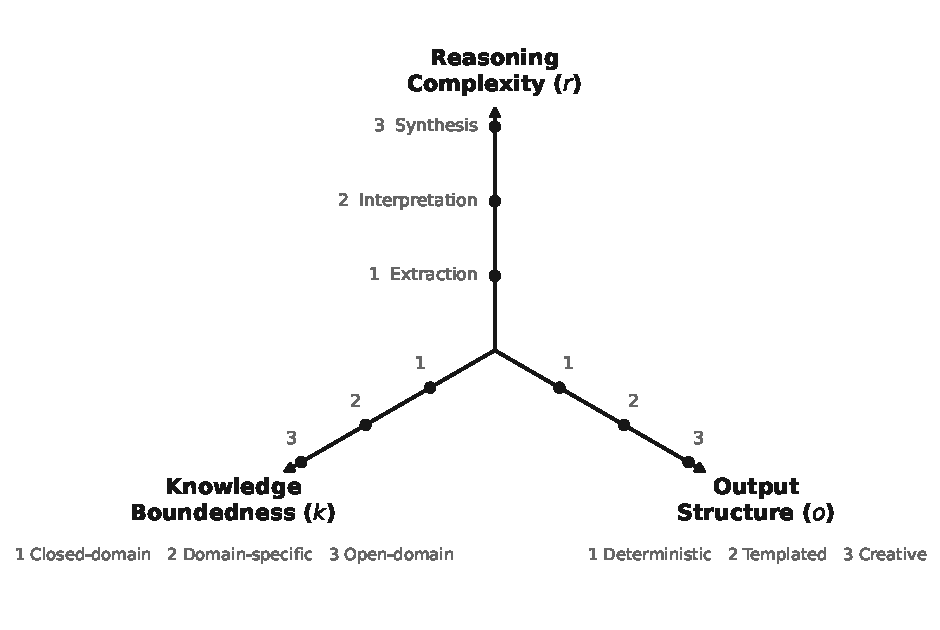
\includegraphics[width=0.82\linewidth]{figure1_axes_schematic}
  \caption{The FIT-SLM-HC task-side coordinate system. The three axes are human-scored task properties on a 1--3 ordinal scale with level~1 being the most constrained (SLM-favorable) level of each axis. This diagram describes tasks only. Whether a given system can cover a given task is settled by measurement (Section~\ref{sec:system}) and not by position in this diagram.}
  \label{fig:framework}
\end{figure}

%% ------------------------------------------------------------
%% SECTION 2.1: TASK-SIDE PROPERTIES
%% ------------------------------------------------------------
\subsection{Task-Side Properties: The 3-Axis Typology}
\label{sec:axes}

Each task is scored on three axes that approximate the cognitive and structural demands it places on a model. Each axis uses a 3-point ordinal scale. The axes are properties of the task alone: they are scored from the task's instructions, inputs, and target outputs without reference to any model.

Scoring should reflect the dominant requirement of the intended workflow under normal operating conditions, not rare edge cases. Reviewers score the task using the actual instructions, input context, and target output expected at deployment. When a task plausibly spans two levels on an axis, the conservative choice is to assign the higher level, or to document both candidate scores and adjudicate explicitly. If retrieval, templating, or other workflow constraints are added before deployment, score the transformed workflow, not the raw prompt alone.

\paragraph{Reasoning Complexity ($r$).}
This axis captures the number of logical steps required to go from input to output. At the lowest level ($r=1$), the answer exists contiguously in the source text and the task is pure extraction (e.g., pulling a patient's age from a clinical note). Moderate complexity ($r=2$) requires interpretation: single-step logic to rephrase or categorize information that is not explicitly labeled, such as classifying a patient portal message as ``urgent'' based on clinical indicators. High complexity ($r=3$) requires synthesis: multi-step reasoning in which the model must connect findings that are not explicitly linked in the input, as in deriving a differential diagnosis. In the technical literature this kind of reasoning is often elicited through ``chain-of-thought'' prompting, in which the model is asked to write out its intermediate reasoning steps before answering \cite{Wei2022, Lievin2024}. Table~\ref{tab:reasoning} summarizes the levels.

\begin{table}[ht]
  \centering
  \caption{Reasoning Complexity ($r$) Scoring Rubric}
  \label{tab:reasoning}
  \begin{tabular}{@{}llll@{}}
    \toprule
    Level & Type & Description & Logic Requirement \\
    \midrule
    $r=1$ & Direct Extraction & Answer exists verbatim in the text & Zero-step (copy/paste) \\
    $r=2$ & Interpretation & Requires rephrasing or categorizing & Single-step logic \\
    $r=3$ & Synthesis & Requires connecting multiple ideas & Multi-step / External logic \\
    \bottomrule
  \end{tabular}
\end{table}

\paragraph{Knowledge Boundedness ($k$).}
This axis measures reliance on stored (internal) knowledge versus provided context. Closed-domain tasks ($k=1$) are self-contained: everything needed to reach an answer is in the prompt \cite{Lewis2020}. Domain-specific tasks ($k=2$) require specialized knowledge not in the prompt, such as clinical terminology, pharmacological interactions, or diagnostic criteria. Open-domain tasks ($k=3$) depend on broad world knowledge or current events \cite{Mallen2023}. Smaller models, whatever their generation, are least disadvantaged on closed-domain tasks, where they function as reasoning engines over the provided data rather than as knowledge stores. Table~\ref{tab:knowledge} summarizes the levels.

\begin{table}[ht]
  \centering
  \caption{Knowledge Boundedness ($k$) Scoring Rubric}
  \label{tab:knowledge}
  \begin{tabular}{@{}llll@{}}
    \toprule
    Level & Type & Information Source & Reliance \\
    \midrule
    $k=1$ & Closed-Domain & Entirely within context window & None (Self-contained) \\
    $k=2$ & Domain-Specific & Specialized or technical knowledge & Moderate (Field-specific) \\
    $k=3$ & Open-Domain & General world knowledge/events & High (External/Stored) \\
    \bottomrule
  \end{tabular}
\end{table}

\paragraph{Output Structure ($o$).}
This axis measures the constraints on what the model must produce. Deterministic outputs ($o=1$) have a fixed format: binary classification, JSON extraction, or predefined labels. Templated outputs ($o=2$) are structured free text that must follow specific stylistic or formatting rules. Creative outputs ($o=3$) are open-ended, and success depends on qualitative factors like tone, empathy, or novelty \cite{Bubeck2023}. Table~\ref{tab:output} summarizes the levels.

\begin{table}[ht]
  \centering
  \caption{Output Structure ($o$) Scoring Rubric}
  \label{tab:output}
  \begin{tabular}{@{}llll@{}}
    \toprule
    Level & Type & Format Style & Primary Evaluation \\
    \midrule
    $o=1$ & Deterministic & Fixed (JSON, Binary, Labels) & Accuracy / Exact Match \\
    $o=2$ & Templated & Constrained free-text & Adherence to Guidelines \\
    $o=3$ & Creative & Open-ended generation & Quality, Tone, \& Novelty \\
    \bottomrule
  \end{tabular}
\end{table}

%% ------------------------------------------------------------
%% SECTION 2.2: SYSTEM-SIDE CAPABILITIES
%% ------------------------------------------------------------
\subsection{System-Side Capabilities: The Envelope}
\label{sec:system}

Task suitability is measured by comparing the local inference stack (model, quantization level, and hardware; Table~\ref{tab:glossary}, Appendix~\ref{app:glossary}) \cite{Dettmers2024} against a reference baseline, preferably a frontier cloud LLM, on two dimensions: accuracy and latency.

The \textbf{Accuracy Ratio (AR)} is the SLM's performance relative to the reference on whatever metric is appropriate for the task (e.g., F1, Recall, BERTScore):
\begin{equation}
  AR = \frac{\text{Performance}_{\text{SLM}}}{\text{Performance}_{\text{Reference}}}
  \label{eq:ar}
\end{equation}

An $AR \geq 1.0$ means the SLM matches or exceeds the reference model; an $AR < 1.0$ quantifies the ``performance tax'' of running on-device. For example, $AR = 0.90$ means the local model retains 90\% of the reference model's score on the chosen metric. In the preferred workflow, the reference is a cloud LLM, though secondary literature analyses may need a stronger non-cloud comparator when no direct cloud baseline exists. This distinction should always be stated, and Section~\ref{sec:vignette-c} shows a case where it reverses the verdict.

Organizations set thresholds based on their own risk threshold. The thresholds used in Section~\ref{sec:snapshot} ($AR \geq 0.90$ primary; $0.80$ lenient; $0.95$ strict) are governance defaults for the framing of this framework and should not be viewed as universal constants. A low-risk administrative task might tolerate moderate AR loss under human review, while a higher-stakes clinical task might demand strict non-inferiority ($AR \geq 0.95$). Because AR is a ratio, comparisons across tasks that use different metric families (e.g., F1, exact match, ROUGE, BERTScore, clinician Likert ratings) are not directly commensurable. Readers should interpret the ratio within the metric it was computed from. Lastly, the Likert-based AR values should be treated as illustrative rather than as a defensible ratio since Likert scales are ordinal.

\textbf{Latency Efficiency (LE)} captures the speed consequence of local execution relative to the incumbent alternative:
\begin{equation}
  LE = 1 - \frac{\text{Latency}_{\text{SLM}}}{\text{Latency}_{\text{Reference}}}
  \label{eq:le}
\end{equation}

For example, $LE = 0.50$ means the local system responds in half the reference's time, and $LE = 0$ means no speed advantage. It is important to note that LE saturates once responses are faster than human perceptual thresholds, at which point further speedup buys little (a point long established in the human--computer interaction literature on absolute response-time limits (roughly 0.1~s for perceived instantaneity, 1~s for uninterrupted flow of thought, 10~s for holding attention)) \cite{Miller1968, Nielsen1993}. It is also important to note that LE penalizes slowdowns more than it credits equivalent speedups (negative values are unbounded). This asymmetry mirrors the general behavioral pattern that losses loom larger than equivalent gains \cite{Kahneman1979, Tversky1991}, and it is consistent with large-scale field experiments in which added delay measurably depressed search use, with effects that outlasted the delay itself \cite{Brutlag2009}.

Because LE is purely relative, it says nothing about whether either system is fast \emph{enough}, as a local model at 0.4~s against a cloud API at 0.2~s scores $LE = -1.0$, though both are imperceptibly fast. While in a different scenario, a local model at 8~s against a 40~s reference scores $LE = 0.80$, both may still be unusable interactively due to the context of the task. The envelope condition therefore also includes an \textbf{absolute latency target} $L_{\max}$, a task-appropriate wall-clock bound chosen by the institution (informed by the thresholds above and by the workflow's tempo) which the candidate system must meet regardless of the ratio. For comparability, LE should be computed using the same latency definition across systems for a given task (e.g., time-to-first-token for interactive generation, or end-to-end completion time for bounded outputs) with repeated trials and reported spread, especially when cloud latency includes network variability.

Together these metrics define the \emph{SLM Capability Envelope}, the set of tasks on which a specific local system meets its risk-adjusted requirements. The envelope should be viewed as a measured set, and not just a read off the task diagram since tasks with equal axis scores may not share a verdict (Figure~\ref{fig:scatter}). The framework keeps these as separate governance signals rather than collapsing them into a single score, because institutions weight safety, privacy, and workflow speed differently depending on the task.

%% ------------------------------------------------------------
%% SECTION 2.3: SCOPE OF CLAIMS
%% ------------------------------------------------------------
\subsection{Scope of Claims: What Is Model-Invariant}
\label{sec:scope}

Any framework evaluated against named models faces a predictable objection: the models will be replaced within months, or even weeks, so why should the findings outlive them? FIT-SLM-HC is structured so that most of it does. Its claims fall into three tiers.

\paragraph{Tier 1: The measurement procedure (model-invariant by construction).}
The task-side axes are scored from the task description, inputs, and target outputs alone. No property of any model enters the scoring. The system-side metrics are ratios defined for an arbitrary pair of systems (any candidate and any reference, including models that do not yet exist), and the envelope thresholds are governance parameters set by the deploying institution.

In addition, nothing in the procedure names a model family, a parameter count, or a benchmark year. Nothing restricts the candidate to being ``small''; formally, the framework compares any candidate system against any reference system, and the SLM-versus-cloud comparison is the motivating instance rather than a structural requirement (the snapshot in Section~\ref{sec:snapshot} already includes a local 8B-versus-70B pair \cite{Builtjes2025}).

\paragraph{Tier 2: A directional mechanism (expected to hold across model generations).}
The further a task moves from simple, self-contained extraction toward open-ended reasoning over stored medical knowledge, the further a smaller model is expected to fall behind its larger reference. The framework predicts that for any \emph{capability-asymmetric} pair (any candidate model less capable than its reference), the candidate's relative performance degrades as a task moves outward along the axes.

The three axes within the FIT-SLM-HC framework are predicted to act through three \emph{different} mechanisms. For the \emph{knowledge axis}, overall model capability is predicted to scale smoothly with parameter count \cite{Kaplan2020}, and the factual knowledge a model can store in its weights also scales with parameter count \cite{AllenZhu2024}. This means a smaller model is at its greatest disadvantage when answers must come from stored knowledge rather than from the prompt. At $k=1$, the prompt itself supplies the knowledge, and the disadvantage is largely neutralized \cite{Lewis2020, Mallen2023}.

For the \emph{reasoning axis}, every added reasoning step compounds the chance of error, and smaller models lose more accuracy on multi-step reasoning than larger ones do \cite{Wei2022, Dziri2023}, so the capability gap widens with $r$.

Lastly, on the \emph{output axis}, constrained outputs (labels, codes, fixed fields) are easier for any model to produce and easier to score, muting the gap at $o=1$ relative to open-ended generation. This remains \emph{untested} by the following snapshots provided in Section~\ref{sec:snapshot}.

\paragraph{Tier 3: A time-indexed snapshot (expected to date).}
The retrospective application in Section~\ref{sec:snapshot} provides an empirical snapshot of healthcare benchmarks published between 2024 and 2026 using the models those studies evaluated. The snapshot demonstrates the framework, and provides a descriptive, non-confirmatory assessment of it.

%% ============================================================
%% SECTION 3: ILLUSTRATIVE APPLICATIONS
%% ============================================================
\section{Illustrative Applications: A 2024--2026 Snapshot}
\label{sec:snapshot}

This section applies FIT-SLM-HC retrospectively to published healthcare benchmarks to show how the framework behaves in real-world cases. Three detailed vignettes are presented: one task inside the envelope with both metrics measurable (Section~\ref{sec:vignette-a}), one outside on the clinically conservative metric (Section~\ref{sec:vignette-b}), and one in which the choice of reference standard flips the verdict (Section~\ref{sec:vignette-c}).

An extended retrospective application to twenty-two tasks across eleven benchmarks follows and is presented descriptively with a full set of sensitivity analyses (formal association tests are confined to Appendix~\ref{app:tests}, labeled exploratory).

It is important to highlight that these applications are illustrative rather than confirmatory. The framework's designer (HW) performed the task scoring initially with outcome values visible, so the patterns show how the framework organizes known evidence and should not be viewed as an independent validation (Sections~\ref{sec:methods-retro} and~\ref{sec:results}, and Limitations, Section~\ref{sec:discussion}).

%% ------------------------------------------------------------
%% SECTION 3.1: METHODS
%% ------------------------------------------------------------
\subsection{Methods for the Retrospective Application}
\label{sec:methods-retro}

\paragraph{Study identification.}
Published healthcare benchmarks comparing SLM(s) and a larger reference model on the same task were identified through a non-systematic convenience search of PubMed, arXiv, and Google Scholar between September 2024 and April 2026, using combinations of ``small language model,'' ``clinical,'' ``biomedical,'' ``on-device,'' ``local deployment,'' and names of specific SLMs (e.g., Phi, Llama-3 8B, Gemma, Qwen).

Inclusion required (a) at least one reported SLM-scale model ($\leq$~9B parameters, the operational cutoff adopted for this snapshot under the functional definition in Section~\ref{sec:intro}), (b) a cloud-scale or larger reference model evaluated on the same task under comparable conditions, and (c) numerical reporting to compute AR.

Studies reporting only aggregate leaderboard scores without task-level splits, studies not primarily in healthcare, and studies without a comparator were excluded. This procedure is thus a convenience-based retrospective mapping and should not be interpreted as a systematic review.

\paragraph{Structure of the resulting sample.}
The 22 unique tasks cluster heavily by source, with one study (MedS-Bench \cite{Wu2025MedS}) contributing seven tasks, and three further studies contributing two or three tasks each. The following data is thus descriptive and the sensitivity analyses in Section~\ref{sec:results} quantify how much each source cluster drives the overall aggregate-level picture.

\paragraph{Axis scoring and blinding status.}
Each task was scored on $(r, k, o)$ by the manuscript author using the rubrics (Section~\ref{sec:axes}) based on the task description, example inputs, and target outputs. When a source reported multiple tasks each task was scored separately. Ambiguous cases were scored conservatively (the higher level on the disputed axis). Two caveats about this scoring approach are important to highlight. First, it is single-rater and the rater is the framework's designer. Second, the original scoring pass, the one used in Table~\ref{tab:extended}, was performed with the source studies' results in view so it was \emph{not} blind to the outcomes it is compared against.

To audit the procedure, the same author re-scored all axis-scoreable tasks against only the task descriptions several days later without reference to the original scores or any AR values. This outcome-blind second pass is used in Section~\ref{sec:results} both as a stability check and as an alternative scoring under which patterns are reassessed. Neither approach, though, substitutes for a blinded multi-annotator method that remains for future work. All data, scoring files, and analysis scripts are provided in the companion repository (see the Data Availability statement).

\paragraph{Analysis.}
The primary analysis is descriptive with mean, median, and range of AR by axis sum and separately by $r$ and $k$ level, with envelope membership counted at $AR \geq 0.80/0.90/0.95$. Because no institutional latency target can be supplied retrospectively, snapshot verdicts apply the accuracy criterion (Equation~\ref{eq:ar}), while the absolute latency target ($L_{\max}$) is checked later at deployment because each institution sets its own speed requirement.

Sensitivity analyses were performed to test whether the main patterns hold under (a) the outcome-blind re-score, (b) leave-one-study-out deletion, (c) every possible one-task-per-study subsample, (d) removal of the two axis-sum-7 tasks, and (e) removal of the MedS-Bench cluster. The scoring audit reports agreement, $\kappa$, the direction of all disagreements with an exact sign test, and Bowker's test of marginal homogeneity \cite{Bowker1948}.

Formal association tests are reported in Appendix~\ref{app:tests} and are exploratory.

%% ------------------------------------------------------------
%% SECTION 3.2: VIGNETTE A
%% ------------------------------------------------------------
\subsection{Vignette A: Inside the Envelope (Pathology Structured-Data Extraction)}
\label{sec:vignette-a}

The first case is extraction of structured parameters from free-text pathology reports \cite{Grothey2025}, the only task in the snapshot for which both AR and LE are computable. The model receives a pathology report and must populate a fixed set of fields. Under FIT-SLM-HC the task scores $(1, 2, 1)$: reasoning is extraction ($r=1$), the vocabulary is specialist pathology terminology ($k=2$), and the output is a deterministic structure ($o=1$).

For this study, the Llama3-8B model reached 91\% overall accuracy against GPT-4's reported ``over 97\%,'' giving $AR = 91/97 = 0.94$ (using the more conservative figure-panel value of 98\% would give 0.93; the verdict is identical at every threshold used here). The authors also report processing times for both systems: 5--6 seconds per report for the local model against approximately 12 seconds per report for GPT-4, giving $LE \approx 0.50$--$0.58$. They concluded that the local 8B model kept about 94\% of the cloud model's accuracy while returning results in roughly half the time, without PHI transmission. At the default governance threshold ($AR \geq 0.90$) the task is inside the envelope, but under strict non-inferiority ($AR \geq 0.95$) it is not. That flip is not a defect of the FIT-SLM-HC framework but a sign of it doing its job, making explicit that the deployment decision here belongs to the institution's risk appetite and not to any benchmark.

The same source then shows how quickly a configuration change can move a task outside the envelope. Quantizing the same model to 4-bit precision dropped accuracy from 91\% to 69\%, i.e.\ $AR = 0.71$, below even the lenient threshold (a chain-of-verification prompting strategy recovered part of the loss, to 73\%). Quantization, hardware, and prompting strategy are all part of the system-side configuration, and Table~\ref{tab:extended} therefore carries the 4-bit variant as its own evaluation row: an envelope verdict certifies a configuration, not a model name.

%% ------------------------------------------------------------
%% SECTION 3.3: VIGNETTE B
%% ------------------------------------------------------------
\subsection{Vignette B: Outside the Envelope (MIMIC-IV Clinical Note Summarization)}
\label{sec:vignette-b}

The second case is extractive summarization of discharge summaries from the MIMIC-IV clinical database \cite{Naemi2025}. The benchmark processed 30{,}000 discharge summaries (averaging 1{,}602 words each) using 16 language models without task-specific fine-tuning. The model must extract and retain all relevant clinical details, including demographics, diagnoses, medications, lab results, procedures, and discharge instructions, and organize them into a structured narrative. Under FIT-SLM-HC, this task scores $(2, 1, 2)$: the model must decide what matters across heterogeneous sections ($r=2$), everything to be summarized is in the note itself ($k=1$), and the summary must follow a structured clinical format while producing natural language ($o=2$).

The comparison here is LLaMa-3-8B on a local NVIDIA A100 GPU (a data-center-class graphics processing unit) against GPT-4o via cloud API. Against GPT-4o, the results split sharply by metric. On ROUGE-1 (unigram content recall), LLaMa-3-8B scored 0.535 versus 0.731, for an $AR = 0.73$. On BERTScore F1 (semantic similarity), it scored 0.828 versus 0.841, an $AR = 0.98$. On reported timing, the local model processed each note in 5.49 seconds versus 10.98 seconds for the cloud API ($LE = 0.50$).

The gap between content recall ($AR = 0.73$) and semantic similarity ($AR = 0.98$) illustrates why metric selection is a governance decision with clinical consequences. For clinical summarization, where a missed medication or allergy in a discharge summary carries direct patient safety risk, content completeness (ROUGE-1) is arguably the more relevant standard, and under it FIT-SLM-HC places the task outside the envelope despite the latency advantage and semantic near-parity. For lower-risk uses where the overall gist matters more than exhaustive detail, the BERTScore AR suggests viability under human review. The contrast with Vignette~A is the framework's intended discriminative behavior: a $(1,2,1)$ extraction task holds 94\% of the reference's accuracy, while a $(2,1,2)$ summarization task loses 27\% of its content recall.

%% ------------------------------------------------------------
%% SECTION 3.4: VIGNETTE C
%% ------------------------------------------------------------
\subsection{Vignette C: The Reference Standard Flips the Verdict (Wearable Fatigue Prediction)}
\label{sec:vignette-c}

The third case is a fatigue prediction task from wearable data (HealthSLM-Bench \cite{Wang2025}). The model receives a 14-day window of Fitbit features and must output a single ordinal label (1--5). The task occupies the most constrained cell of the task space, $(1,1,1)$: pattern matching over structured numeric inputs ($r=1$), fully within the context window ($k=1$), deterministic output ($o=1$). By the Tier-2 mechanism this is exactly where an SLM should be most competitive, and the benchmark's zero-shot results bear that out in one direction while complicating it in another.

Against the larger \emph{on-device} comparator in the benchmark (Llama-2-7B, 41.2\% accuracy), the best zero-shot SLM (Phi-3-mini-4k, 62.9\%) achieves $AR = 1.53$, so on-device small beats large. The same source however also evaluated cloud models zero-shot, and GPT-4 reached 72.2\% (GPT-3.5: 70.8\%), so against the framework's preferred cloud reference the same SLM scores $AR = 62.9/72.2 = 0.87$, below the 0.90 default threshold and inside only the lenient 0.80 envelope.

On latency, they report time-to-first-token for on-device models only (6.39~s for Phi-3-mini-4k versus 29.12~s for Llama-2-7B on an iPhone 15 Pro Max) with no cloud latency reported.

The point of this vignette is that the same result can look strong or weak depending on the reference model chosen. Referencing the larger on-device alternative versus the best available cloud model turns $AR = 1.53$ into $AR = 0.87$ on identical outputs, which means converting a 53\% advantage into a 13\% deficit. An institution whose realistic alternative is a cloud API should compute AR against the cloud model, and one whose alternative is a larger on-device model (for connectivity, cost, or policy reasons) should compute it against that.

%% ------------------------------------------------------------
%% SECTION 3.5: EXTENDED APPLICATION
%% ------------------------------------------------------------
\subsection{Extended Application Across Published Benchmarks}
\label{sec:extended}

The three vignettes were chosen to illustrate boundary cases, so by themselves they cannot show how the framework behaves across the published literature more broadly. The snapshot below therefore asks across the benchmarks identified in Section~\ref{sec:methods-retro}, do the three task axes separate the places where small models keep up from the places where they fall short? To fill that gap and further characterize the framework's behavior beyond the three vignettes, FIT-SLM-HC was applied retrospectively to 22 unique healthcare tasks from 11 recent benchmark studies using the identification and scoring procedure described in Section~\ref{sec:methods-retro}.

For each task, the best-performing SLM and a cloud or larger reference model from the published results were identified, and the Accuracy Ratio was computed. Where inference latency was reported for both systems, Latency Efficiency was also computed. One study \cite{Grothey2025} additionally reported a 4-bit quantized variant of the same task, which is retained in Table~\ref{tab:extended} as a separate row (marked with $^c$) to illustrate configuration-level effects, yielding 23 evaluation rows in total. Table~\ref{tab:extended} reports the results.

\begin{table}[p]
\centering
\scriptsize
\setlength{\tabcolsep}{3.5pt}
\renewcommand{\arraystretch}{0.91}
\caption{Extended FIT-SLM-HC application: 22 unique healthcare tasks from 11 benchmarks (23 rows; the marked row is a quantization variant) ordered by axis sum. AR = Accuracy Ratio (SLM $\div$ Reference); LE = Latency Efficiency; NR = not reported. Reg.\ = reference regime: ZS zero-shot, 3S 3-shot, FT fine-tuned, P prompted (shots not stated). Env.\ = verdict at the default $AR \geq 0.90$ in the source configuration ($\checkmark$ inside, $\times$ outside); sensitivity at 0.80/0.95 in Section~\ref{sec:results}.}
\label{tab:extended}
\begin{tabular}{@{}p{2.05cm}lp{1.45cm}p{1.25cm}cccrrccl@{}}
\toprule
Task & Source & SLM & Ref. & Reg. & $(r,k,o)$ & Metric & SLM & Ref. & AR & LE & Env. \\
\midrule
\multicolumn{12}{@{}l}{\textit{Low complexity ($r{+}k{+}o = 3$)}} \\
Report labeling & \cite{Zheng2026} & OPT-350M & GPT-4o & P & (1,1,1) & F1 & .894 & .728 & 1.23 & NR & $\checkmark$ \\
Text classif. & \cite{Wu2025MedS} & Llama3-8B$^a$ & GPT-4 & 3S & (1,1,1) & F1 & 86.7 & 68.1 & 1.27 & NR & $\checkmark$ \\
Info. extraction & \cite{Wu2025MedS} & Llama3-8B$^a$ & GPT-4 & 3S & (1,1,1) & Acc & 83.8 & 76.9 & 1.09 & NR & $\checkmark$ \\
Stress detection & \cite{Hanafi2024} & Gemma 2 9B & GPT-4 & P & (1,1,1) & Acc & 72 & 70 & 1.03 & NR & $\checkmark$ \\
\multicolumn{12}{@{}l}{\textit{Low--moderate complexity ($r{+}k{+}o = 4$)}} \\
DICOM harmoniz. & \cite{Zheng2026} & OPT-350M & GPT-4o & P & (1,2,1) & Acc & .975 & .878 & 1.11 & NR & $\checkmark$ \\
Clinical NER & \cite{Wu2025MedS} & Llama3-8B$^a$ & GPT-4 & 3S & (1,2,1) & F1 & 79.3 & 59.5 & 1.33 & NR & $\checkmark$ \\
Pathology IE & \cite{Grothey2025} & Llama3-8B & GPT-4 & P & (1,2,1) & Acc & 91 & 97$^g$ & 0.94 & 0.54$^h$ & $\checkmark$ \\
Pathology IE$^c$ & \cite{Grothey2025} & Llama3-8B 4-bit & GPT-4 & P & (1,2,1) & Acc & 69 & 97$^g$ & 0.71 & NR & $\times$ \\
Clinical report IE & \cite{Liu2025ClinIE} & Llama-3.1-8B$^d$ & GPT-4 & ZS & (1,2,1) & EM & 90.0 & 86.1 & 1.05 & NR & $\checkmark$ \\
Biomed.\ CLS (binary) & \cite{Dawood2025} & Qwen2.5-7B & Gemini 2.5 & P & (1,2,1) & Acc & 92 & 90 & 1.02 & NR & $\checkmark$ \\
Depression detect. & \cite{Hanafi2024} & Gemma 2 9B & GPT-4 & P & (2,1,1) & Acc & 80.4 & 85.0 & 0.95 & NR & $\checkmark$ \\
Suicide detect. & \cite{Hanafi2024} & Llama3-8B & GPT-4 & P & (2,1,1) & Acc & 58 & 70 & 0.83 & NR & $\times$ \\
\multicolumn{12}{@{}l}{\textit{Moderate complexity ($r{+}k{+}o = 5$)}} \\
Impression gen.$^e$ & \cite{Zheng2026} & OPT-350M & GPT-4o & P & (2,1,2) & Likert & 4.39 & 3.65 & 1.20 & NR & $\checkmark$ \\
Diagnosis (DDXPlus) & \cite{Wu2025MedS} & Llama3-8B$^a$ & GPT-4 & 3S & (2,2,1) & Acc & 97.5 & 58.1 & 1.68 & NR & $\checkmark$ \\
Treatment plan. & \cite{Wu2025MedS} & Llama3-8B$^a$ & GPT-4 & 3S & (2,2,1) & Acc & 98.5 & 84.7 & 1.16 & NR & $\checkmark$ \\
ICD-10 coding & \cite{Hou2025} & Llama-1B$^b$ & GPT-4o mini$^b$ & FT & (2,2,1) & EM & $\sim$93 & $\sim$90 & $\approx$1.03 & NR & $\checkmark$ \\
Radiology QA & \cite{Ranjit2024} & RadPhi-3 3.8B & GPT-4 & P & (2,2,1) & F1 & 40.3 & 34.0 & 1.19 & NR & $\checkmark$ \\
DDI prediction & \cite{DeVito2025} & Phi-3.5 2.7B$^d$ & GPT-4o & P & (2,2,1) & Acc & .913 & .926 & 0.99 & NR & $\checkmark$ \\
Biomed.\ CLS (3-class) & \cite{Dawood2025} & Llama3-8B & Gemini 2.5 & P & (2,2,1) & Acc & 70 & 90 & 0.78 & NR & $\times$ \\
\multicolumn{12}{@{}l}{\textit{High complexity ($r{+}k{+}o \geq 6$) and composite}} \\
Clinical triage & \cite{Wu2025MedS} & Llama3-8B$^a$ & GPT-4 & 3S & (3,2,1) & Acc & 63.1 & 60.1 & 1.05 & NR & $\checkmark$ \\
Clinical IE (28)$^f$ & \cite{Builtjes2025} & Llama-3.1-8B & Llama-3.3-70B & ZS & (var.) & Utility & .588 & .760 & 0.77 & NR & $\times$ \\
Medical exam QA & \cite{Kim2025} & Meerkat-7B & GPT-4 & P & (3,3,1) & Acc & 64.5 & 76.6 & 0.84 & NR & $\times$ \\
Medical QA (USMLE) & \cite{Wu2025MedS} & Llama3-8B$^a$ & GPT-4 & ZS & (3,3,1) & Acc & 63.6 & 85.8 & 0.74 & NR & $\times$ \\
\bottomrule
\multicolumn{12}{@{}p{15.6cm}}{\scriptsize $^a$MMedIns-Llama 3-8B instruction-tuned on the MedS-Ins corpus whose task categories include those of the evaluation benchmark (Section~\ref{sec:methods-retro}). AR in these rows may partly reflect task-family exposure. $^b$Both models fine-tuned, with AR approximate across test subsets. $^c$4-bit quantized variant of the same task and system and not counted as a unique task. $^d$Fine-tuned with LoRA. Model names/sizes are as printed in each source (e.g., ``Phi-3.5 2.7B'' is the DDI source's naming). $^e$Likert is ordinal so this AR (a ratio of mean ratings) is illustrative only. $^f$Composite DRAGON ``utility'' score over 28 heterogeneous Dutch-language clinical NLP tasks, no single axis profile and excluded from axis-based analyses. $^g$The source's text reports GPT-4 at ``over 97\%'' (a figure panel shows 98\%, which would give AR 0.93 and 0.70 with identical verdicts). English dataset. $^h$Midpoint of 5--6~s/report (local) vs.\ $\sim$12~s/report (GPT-4); as an interval, $LE = 0.50$--$0.58$.} \\
\end{tabular}
\end{table}

%% ------------------------------------------------------------
%% SECTION 3.6: RESULTS
%% ------------------------------------------------------------
\subsection{Descriptive Results and Sensitivity Analyses}
\label{sec:results}

\begin{figure}[ht]
  \centering
  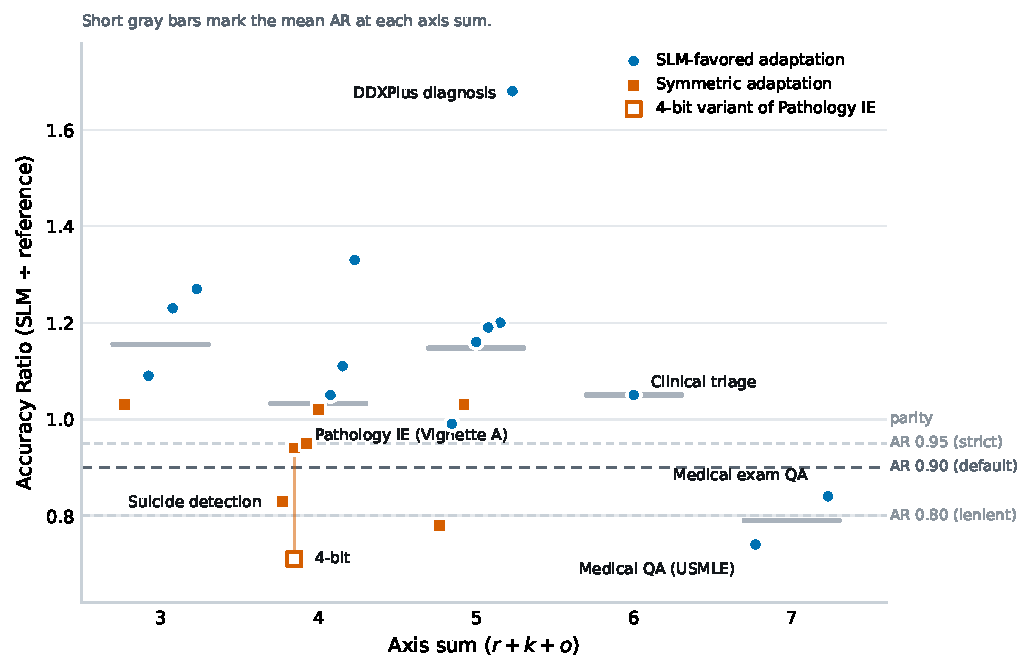
\includegraphics[width=0.98\linewidth]{figure2_ar_scatter}
  \caption{Accuracy Ratio against axis sum for the 21 axis-scored unique snapshot tasks (the composite row of Table~\ref{tab:extended} has no single axis profile and is not shown). Short gray bars mark the mean AR at each axis sum, with dashed lines marking the three governance thresholds.}
  \label{fig:scatter}
\end{figure}

Of the 18 unique tasks with axis sum $\leq 5$, 16 reached $AR \geq 0.90$ and 13 exceeded 1.0. In 11 of the 13, a fine-tuned or instruction-tuned SLM matched or beat a cloud-scale model outright, and in the remaining two a prompted-only SLM did. The most consistent results came from the most constrained tasks: report labeling, text classification, clinical named-entity recognition (NER; tagging mentions of drugs, diagnoses, and findings in text), and information extraction, all of which involve pulling structured outputs from the provided context. The three unique tasks at axis sum $\geq 6$ split one inside (clinical triage, $AR = 1.05$) and two outside (the exam-QA tasks, $AR = 0.84$ and $0.74$).

\begin{table}[ht]
\centering
\small
\caption{Descriptive statistics for AR by axis sum (21 axis-scored unique tasks; published pass-1 scores). ``Inside'' counts tasks at or above each AR threshold.}
\label{tab:descriptives}
\begin{tabular}{@{}crccccccc@{}}
\toprule
Axis sum & $n$ & Mean AR & Median & Min & Max & $\geq$0.80 & $\geq$0.90 & $\geq$0.95 \\
\midrule
3 & 4 & 1.16 & 1.16 & 1.03 & 1.27 & 4 & 4 & 4 \\
4 & 7 & 1.03 & 1.02 & 0.83 & 1.33 & 7 & 6 & 5 \\
5 & 7 & 1.15 & 1.16 & 0.78 & 1.68 & 6 & 6 & 6 \\
6 & 1 & 1.05 & 1.05 & 1.05 & 1.05 & 1 & 1 & 1 \\
7 & 2 & 0.79 & 0.79 & 0.74 & 0.84 & 1 & 0 & 0 \\
\bottomrule
\end{tabular}
\end{table}

\paragraph{What the distribution shows.}
Mean AR is flat and unordered across axis sums 3 through 6 (1.16, 1.03, 1.15, 1.05; the mean at sum 5 exceeds the mean at sum 4) and drops only at axis sum 7 (Table~\ref{tab:descriptives} and Figure~\ref{fig:scatter}). What this shows is that a task's axis sum does not predict its AR, and interestingly that the two open-domain medical exam QA tasks sit apart from everything else. Those two tasks are also the only tasks at $k=3$.

Broken out by individual axis, reasoning complexity is the only axis with a level-by-level decline in mean AR (1.12 at $r=1$, 1.09 at $r=2$, 0.88 at $r=3$; $n = 9/9/3$), though the step from $r=1$ to $r=2$ is negligible and two of the three $r=3$ tasks are the same exam-QA pair. Knowledge boundedness shows no clear ordering in the populated range (1.09 at $k=1$, 1.11 at $k=2$; $n = 7/12$) and its $k=3$ level coincides with the exam-QA pair. There is no real variation in output structure to compare (20 tasks at $o=1$, one at $o=2$, none at $o=3$), so the $o$ mechanism of Section~\ref{sec:scope} remains untested.

\paragraph{Threshold sensitivity.}
Because the $AR \geq 0.90$ threshold is a governance choice rather than a universal constant, envelope membership was also computed at $AR \geq 0.80$ and $\geq 0.95$. Across the 22 unique tasks, 19 are inside at $AR \geq 0.80$, 17 at $\geq 0.90$, and 16 at $\geq 0.95$. Among the 18 low-axis tasks the counts are 17, 16, and 15. Two tasks change envelope status between the lenient and default thresholds (suicide detection, $AR = 0.83$; medical exam QA, $AR = 0.84$) and one changes between the default and strict thresholds (Pathology IE, $AR = 0.94$, the Vignette~A case). The overall picture is stable across thresholds, but individual task verdicts depend on where the threshold is set and on whether the underlying comparison was adaptation-symmetric (Table~\ref{tab:extended}).

\paragraph{Sensitivity analyses.}
Table~\ref{tab:sensitivity} recomputes the aggregate association between axis sum and envelope membership guided by Section~\ref{sec:methods-retro}. (Appendix~\ref{app:tests} gives the full versions with confidence intervals.)

\begin{table}[ht]
\centering
\small
\caption{Sensitivity of the axis-sum/envelope association ($AR \geq 0.90$; low = axis sum $\leq 5$, high = $\geq 6$; trend-eligible unique tasks). OR = odds ratio; CA = Cochran--Armitage trend test.}
\label{tab:sensitivity}
\begin{tabular}{@{}lccccc@{}}
\toprule
Analysis & $n$ & Low in/total & High in/total & Fisher $p$ & CA $p$ \\
\midrule
Pass-1 scores (published; not outcome-blind) & 21 & 16/18 & 1/3 & 0.080 & 0.017 \\
Pass-2 scores (outcome-blind re-score) & 21 & 13/15 & 4/6 & 0.544 & 0.028 \\
Axis-sum-7 tasks removed & 19 & 16/18 & 1/1 & 1.000 & 0.676 \\
MedS-Bench cluster removed & 14 & 11/13 & 0/1 & 0.214 & 0.071 \\
\bottomrule
\end{tabular}
\end{table}

The appearance of a strong axis-sum effect in the full sample therefore depends jointly on the non-blind first-pass scores, on the two exam-QA tasks, and on the seven-row MedS-Bench cluster. If one removes any one of these the effect either weakens or disappears (Table~\ref{tab:sensitivity}; leave-one-study-out and one-task-per-study results are given in Appendix~\ref{app:tests}). The claim this snapshot thus supports is descriptive only, that well-defined extraction and classification tasks routinely reach or exceed cloud-reference accuracy under current adaptation practice, while open-domain exam-style QA do not, and the region between them is unordered on present evidence.

Three further observations complete the picture. First, related to scoring audit the outcome-blind re-score agreed with the published scores on 82\% of rows for $r$, 82\% for $k$, and 100\% for $o$ ($\kappa$ = 0.71, 0.63, and 1.00), but all eight disagreements moved scores upward (exact sign-test $p = 0.008$; Bowker's test flags the $k$ axis, $p = 0.046$ \cite{Bowker1948}), a systematic drift concentrated at the $r$~1/2, $r$~2/3, and $k$~1/2 boundaries. While three of the moved tasks cross the axis-sum 5/6 boundary, which is what reverses the association in Table~\ref{tab:sensitivity}, so the rubric language needs sharpening at those boundaries before any multi-annotator study.

Second, task adaptation acts as an envelope expander, where the largest AR values in the snapshot come from task-adapted SLMs compared against prompted references, with the biggest gains in the MedS-Bench cluster (Table~\ref{tab:extended}, note~$a$). One of the two low-axis tasks that fell outside the envelope (suicide-risk detection, $AR = 0.83$) likely depends on implicit language cues that smaller models handle less reliably.

Third, latency reporting is nearly absent. Only one of the thirteen studies reports timing for both systems in a form that supports LE, so the two-metric envelope is exercised end-to-end only in Vignette~A and the extended analysis is effectively accuracy-only, a field-wide reporting gap that Section~\ref{sec:discussion} proposes to fix.

%% ============================================================
%% SECTION 4: DISCUSSION AND CONCLUSION
%% ============================================================
\section{Discussion and Conclusion}
\label{sec:discussion}

FIT-SLM-HC rests on the claim that language model deployment decisions in healthcare depend less on model size than on whether the task's constraints match the system's capabilities. The snapshot in Section~\ref{sec:snapshot} shows the framework organizing current evidence in a way that is useful and explicit about limitations: (1) well-defined extraction and classification tasks routinely reach cloud-reference accuracy while open-domain exam-style QA does not, (2) the reasoning axis carries the clearest per-axis gradient, and (3) the middle of the task space is unordered on present evidence.

SLMs are not simply weaker versions of cloud models, rather they can function as efficient reasoning engines when given the right context. FIT-SLM-HC is a deployment triage layer on top of broader evaluation work, not a replacement for benchmarking, calibration, or safety assessment.

Model turnover strengthens rather than weakens the case for this kind of framework. A published claim of the form ``model X achieves score Y on task Z'' begins to date the day the next model family ships. Under FIT-SLM-HC, an envelope verdict is explicitly indexed to a task, a system configuration (model, adaptation, quantization, hardware), a reference standard, a set of governance thresholds, and a measurement date. Vignette~C makes the reference-standard index concrete, showing that the same model on the same task scores $AR = 1.53$ against its on-device comparator and $0.87$ against the cloud baseline in the same benchmark table.

Institutions should begin, if they don't already, to treat verdicts as perishable measurements to be recomputed when models or hardware change, and not as durable properties of task types. The durable parts of the framework are the measurement procedure and the directional mechanism (Tiers 1 and 2 in Section~\ref{sec:scope}). This aligns with the expectation that improving small models will move the boundary outward.

In practice, the framework comes down to three steps. First, score the candidate task on the $(r, k, o)$ axes, which sets expectations, orders the evaluation queue, and flags where to look hardest. Second, establish a reference standard on a small evaluation set and name the reference deliberately (Vignette~C). Preferably a frontier cloud LLM under deployment conditions is used for the reference, or where the realistic alternative is different, the alternative is clearly labeled. Third, run the candidate system on the same set and compute AR, LE, and the absolute latency check. The measurement in steps two and three renders the verdict; deploy only if the organization's thresholds are met.

To make this procedure easier to apply, a companion open-source web tool \cite{Williams2026FITSLMHCTool} walks users through all three steps as an interactive static-site application. No server is needed. Users score a candidate task on the $(r, k, o)$ axes, enter their SLM and reference model performance numbers, and optionally provide latency data. The tool computes AR and LE in real time, plots the user's task alongside the snapshot tasks of Table~\ref{tab:extended}, and returns an envelope verdict against adjustable governance thresholds (inside; borderline, meaning within 0.05 below the AR threshold; or outside).

Because the tool runs entirely client-side with no data leaving the browser, it is usable in institutional environments with strict data transmission policies, and because its inputs are user-supplied measurements rather than stored model profiles, it remains usable as new models are released. The tool is a first-pass triage aid, and does not replace the benchmarking and safety assessment that should follow a positive envelope verdict.

Lastly, healthcare has several features that make this kind of structured assessment particularly necessary. The compliance picture is more nuanced than a simple local-versus-cloud dichotomy. As noted previously in Section~\ref{sec:intro}, cloud LLM endpoints can be operated under a Business Associate Agreement \cite{HHSBAA, Marks2023HIPAAAI}, and de-identification pipelines can strip PHI before cloud transmission for certain task types \cite{Kovacevic2024DeID}. Equally, local SLM deployment can eliminate the transmission vector but does not automatically make it compliant: the HIPAA Security Rule still requires access controls, encryption, audit logging, and workforce training on any system that touches PHI \cite{HHS2013SecurityRule}.

FIT-SLM-HC does not make compliance determinations, but its primary role is to quantify the performance side of the trade-off so that organizations can make an informed decision about whether the local model is accurate and fast enough for the task at hand. The clinical risk spectrum is also wide, as an SLM prediction error on a wearable wellness score is not equivalent to a missed medication in a discharge summary. The framework keeps those concerns separate as the axis scores capture the capability demand of the task, while the clinical stakes enter through where the institution sets its AR threshold and its metric (Vignette~B). Healthcare workflows also frequently include human review, which can compensate for moderate AR deficits on lower-risk tasks. The framework accommodates this by letting organizations set thresholds based on how feasible human-in-the-loop oversight is for a given task.

\paragraph{Limitations.}
The axis scoring is currently single-rater. A blinded multi-annotator study, with rubric language sharpened at the $r$~1/2, $r$~2/3, and $k$~1/2 boundaries, is required before the axis scores can be treated as measurements. The 11 source studies were identified by convenience search, with the 22 tasks clustered by source (seven from one study and one SLM checkpoint). Most SLM entries are fine-tuned or instruction-tuned against prompted references (3-shot GPT-4 in the largest cluster), and the instruction corpus of that cluster's SLM overlaps the benchmark's task families with no held-out protocol described. This means the largest AR values may partly reflect task exposure. AR is also computed across incommensurable metric families (F1, accuracy, exact match, ROUGE-1, BERTScore, Likert, a composite utility), Likert-based AR in particular is illustrative only, and the composite Dutch-language row aggregates 28 heterogeneous tasks. Usable LE exists for one extended-table task, so the two-dimensional envelope is exercised only in Vignette~A, and the vignettes use heterogeneous hardware and latency definitions. Finally, extending the framework to cost, energy, and subgroup fairness reporting, and evaluating how retrieval augmentation, structured prompting, and abstention policies reshape effective task coordinates, are potential next steps.

The framework is also deliberately limited in scope. It does not treat cost, energy, security, or equity as co-equal quantitative axes, and it does not collapse AR and LE into a single utility score. Those factors matter in healthcare governance, but the aim here is a simple first-pass decision structure that institutions can layer with their own policy, procurement, and safety requirements.

\paragraph{Latency reporting in healthcare AI benchmarks.}
FIT-SLM-HC treats AR and LE as co-equal governance signals, yet only one of the thirteen studies examined reports timing for both systems in a form that allows LE computation, and only two others report timing for even one side of the comparison. In healthcare, where response time affects clinical workflow integration, patient throughput, and clinician trust, this omission matters. Future healthcare AI benchmarks should report, at minimum, the median and interquartile range of per-query wall-clock time (or tokens per second) for each model, under a stated measurement setting and matched input conditions, alongside the accuracy metrics already considered standard. Until this happens, half of the FIT-SLM-HC decision surface will remain empirically inaccessible.

\paragraph{Conclusion.}
To conclude, FIT-SLM-HC extends evaluation beyond purely technical accuracy benchmarks to task-level assessment of on-device language models in healthcare. By separating task properties from system metrics, separating what is model-invariant from what is a dated measurement, and insisting that the reference standard, the metric, and the thresholds be named, it gives organizations a way to deploy SLMs where they add value (preserving privacy and cutting cost), to avoid them where they would introduce clinical risk, and to remake that decision each time the available models change.

%% ============================================================
%% DECLARATIONS
%% ============================================================
\section*{Declarations}

\subsection*{Funding}
This work received no specific funding from any public, commercial, or not-for-profit agency.

\subsection*{Competing Interests}
The author declares no competing interests.

\subsection*{Ethics Approval}
Not applicable. This study analyzed previously published, aggregate benchmark results; no human participants, patient records, or identifiable data were involved.

\subsection*{Author Contributions}
H.W.\ conceived the framework, performed the literature identification and task scoring, conducted the analyses, developed the companion tool, and wrote the manuscript.

\subsection*{Use of Artificial Intelligence}
Generative AI (Anthropic Claude) assisted with drafting, reference verification, and figure generation; the author verified all content and takes full responsibility.

\subsection*{Data Availability}
No new clinical data were collected for this study; all performance figures are drawn from previously published benchmark results cited in the text. All materials supporting this paper are in a single public repository at \url{https://github.com/hantswilliams/fit-slm-hc}: the manuscript source (\texttt{manuscript/}), the analysis scripts, both scoring passes, the sensitivity suite, and all generated outputs supporting Section~\ref{sec:snapshot} (\texttt{analysis/}), a bibliography verification script, and the companion FIT-SLM-HC decision tool (\texttt{docs/}), an open-source static web application whose live, browser-based version is deployed at \url{https://hantswilliams.github.io/fit-slm-hc/}. Earlier drafts and additional exploratory materials from the framework's development are held in a separate private working repository and are available from the author on reasonable request.

%% ============================================================
%% APPENDICES
%% ============================================================
\appendix
%% Appendix tables are numbered by appendix letter (A1, B1, ...), separate from the main-text sequence.
\renewcommand{\thetable}{\Alph{section}\arabic{table}}
\setcounter{table}{0}

\section{Exploratory Association Tests}
\label{app:tests}

This appendix reports the formal association statistics between axis sum and envelope membership. They are labeled exploratory because three conditions for valid inference fail here: the observations cluster by source study (Section~\ref{sec:methods-retro}), the published axis scores were not assigned blind to the outcome, and the high-axis region contains too few tasks for the tests to be stable (Table~\ref{tab:sensitivity}). Two tests of the same hypothesis are shown, which is itself a multiplicity the reader should keep in view; their disagreement in the full sample (the trend test is more sensitive precisely because it leans on the sparse ordered tail) is diagnostic of that fragility.

Each analysis dichotomizes tasks at axis sum $\leq 5$ versus $\geq 6$ and at $AR \geq 0.90$, and reports a two-sided Fisher exact test, an odds ratio with a Woolf 95\% confidence interval (Haldane--Anscombe 0.5 correction when a cell is zero), and a Cochran--Armitage trend test across ordered axis sums. On the published pass-1 scores, the full trend-eligible sample ($n = 21$) gives Fisher $p = 0.080$ with $OR = 16.0$ (95\% CI $[0.96,\,267.0]$, crossing 1) and Cochran--Armitage $z = -2.39$, $p = 0.017$. In the SLM-favored stratum ($n = 14$): Fisher $p = 0.033$, $OR = 38.3$ (corrected 95\% CI $[1.18,\,1245.0]$), $z = -2.73$, $p = 0.006$. In the symmetric stratum ($n = 7$) no high-axis comparisons exist in the sampled literature, so the $2{\times}2$ statistics are not computable; the trend test across the observed axis sums (3, 4, 5) gives $z = -0.94$, $p = 0.35$, against mean AR of 1.03, 0.94, and 0.91. The extremely wide confidence intervals are the arithmetic signature of the sparse high-axis cells. Under the outcome-blind pass-2 scores the full-sample statistics become Fisher $p = 0.544$, $OR = 3.25$, $z = -2.20$, $p = 0.028$; removing the two axis-sum-7 tasks leaves $z = -0.42$, $p = 0.68$ (Table~\ref{tab:sensitivity}). Leave-one-study-out deletion leaves the Fisher $p$ above 0.05 in every one of the ten study-deletion subsets (range 0.051--0.284), with the trend statistic weakening most when the exam-QA study (CA $p = 0.086$) or the MedS-Bench cluster (CA $p = 0.071$) is removed; across all 126 one-task-per-study subsamples (10 tasks each), the trend $p$-value has median 0.036 (range 0.004--0.440) and falls below 0.05 in 78 of 126, while the Fisher $p$ has median 0.20. Regenerated outputs for every analysis in this appendix, including the leave-one-study-out and one-task-per-study enumerations, are in \texttt{aug28/analysis/outputs/} in the companion repository.

\section{Key Terms Reference}
\label{app:glossary}

Table~\ref{tab:glossary} defines the model and metric terms used throughout the paper.

\begin{table}[ht]
\centering
\small
\caption{Key terms as used in this paper.}
\label{tab:glossary}
\begin{tabular}{@{}p{3.4cm}p{11.4cm}@{}}
\toprule
Term & Meaning here \\
\midrule
LLM / SLM & Large language model (typically cloud-hosted; ``frontier'' denotes the most capable current generation) / small language model, defined functionally above as one that runs on institution-controlled hardware. \\
Parameter (weight) & One of the internal numerical values a model learns during training. Parameter count is the standard measure of model size; ``weights'' is a synonym. \\
Token & A short chunk of text, roughly a word or word fragment, that a model reads and writes one at a time. \\
Inference & Running a trained model to produce an output for a given input. Cloud providers typically charge per inference. \\
Hallucination & Fluent but factually incorrect or fabricated model output; the main reason model outputs in healthcare require human verification. \\
Zero-shot / few-shot & Using a model with instructions only (zero-shot), or with a small number of worked examples included in the prompt (few-shot; ``3-shot'' means three examples). \\
Fine-tuning & Additional training of a model on examples of the target task. \\
Instruction tuning & Fine-tuning on instruction--response pairs, often domain-specific (e.g., medical). \\
LoRA & Low-rank adaptation: a lightweight fine-tuning method that trains a small add-on to an otherwise frozen model. \\
Adaptation & Umbrella term for fine-tuning, instruction tuning, or LoRA. A comparison is \emph{symmetric} when both models are comparably adapted (or both merely prompted) and \emph{SLM-favored} when only the small model was adapted for the task. \\
Quantization & Storing model weights at lower numeric precision (e.g., 4-bit) to cut memory use and increase speed, sometimes at an accuracy cost. \\
Parametric knowledge & Facts stored in a model's weights during training, as opposed to information supplied in the prompt. \\
Prompt / context window & The text given to the model at question time / the maximum amount of such text the model can consider at once. \\
Retrieval augmentation & Automatically fetching relevant reference text (e.g., from a document store) and adding it to the prompt, so the model answers from supplied context rather than from stored knowledge. \\
Time-to-first-token & Delay between submitting a request and the start of the model's answer; a common interactive-latency measure. \\
F1 score & Harmonic mean of precision and recall (0--1); balances false positives against false negatives. \\
Exact match (EM) & Fraction of outputs identical to the reference answer. \\
ROUGE-1 & Word overlap between a generated summary and a reference summary; read here as content recall (did the summary keep the source facts?). \\
BERTScore & Similarity of \emph{meaning} between generated and reference text; can stay high even when specific details are missing. \\
Cohen's $\kappa$ & Agreement between two sets of ratings, corrected for chance; 0 = chance-level, 1 = perfect. Reported here without conventional verbal glosses, because both rating passes come from the same rater (Section~\ref{sec:results}). \\
Odds ratio (OR); 95\% CI & How many times higher the odds of an outcome are in one group than another; the confidence interval is the range of values compatible with the data; an interval that crosses 1 means ``no effect'' cannot be ruled out. \\
\bottomrule
\end{tabular}
\end{table}
\clearpage  % flush the glossary table before the reference list

%% ============================================================
%% REFERENCES
%% ============================================================
\bibliographystyle{unsrtnat}
\bibliography{references}

\end{document}
